\section{Dynamical Systems Model of the Oil Economy}
\label{sec: model}

\begin{figure}
    \centering
    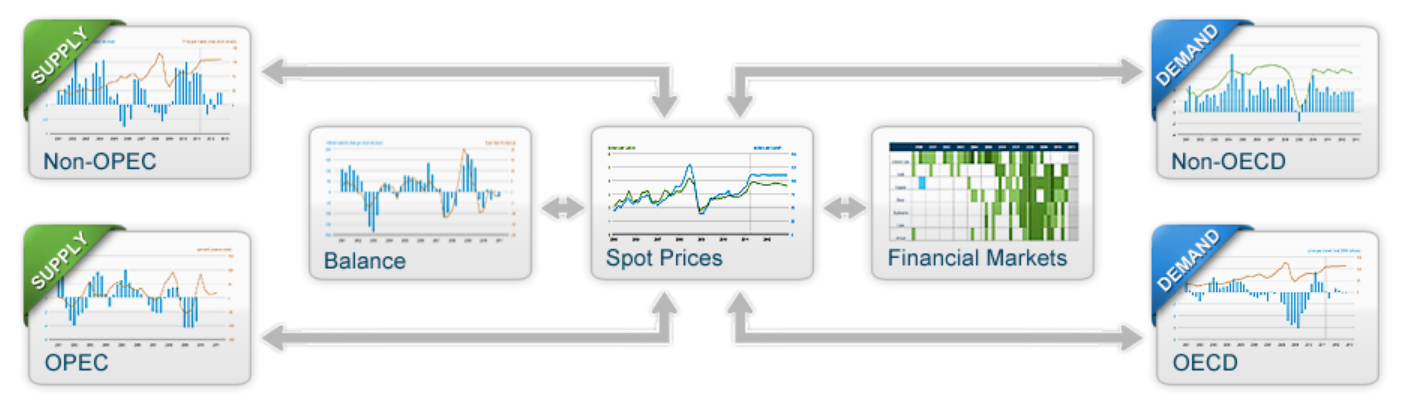
\includegraphics[width=.5\textwidth]{Figures/oilmarketscheme.PNG}
    \caption{Schematic view of what drives oil prices [eia].}
    \label{fig:EIAmodel}
\end{figure}



\subsection{Model Assumptions} 
\begin{itemize}
    \item Inelastic, unknown OPEC Supply
    \item Elastic non-OPEC Supply
    \item Ignore Lead Time
    \item All oil is fungible
    \item Linear aggregation producers
    \item Linear aggregation consumers
    \item market price equals competitive production cost
    \item Ignore Futures Market
    \item Ignore Economic Growth (pre filtered)
    \item Ignore capacity constraints
\end{itemize}

\begin{figure}
    \centering
\begin{tikzpicture}[every node/.style={bgelement},every edge/.append style={bond}]
\node at (0,0) (0junc) {0};
\node at (0,1) (up) {};
\node[label=left:$non-OPEC$,left=1 of up] (nOPEC) {I};
\node[label=right:$non-OECD$,right=1 of up] (nOECD) {$\textbf{S}_f$};
\node[label=right:$OECD$,below=1 of nOECD] (OECD) {I};
\node[label=left:$OPEC$,below=1 of nOPEC] (OPEC) {$\textbf{S}_f$};
\node[label=below:$e$,below=1 of 0junc] (1junc) {1};
\node[label=left:$Balance$,left=1 of 1junc] (C) {C};
\node[label=right:$Fin.\ markets$,right=1 of 1junc] (R) {R};
\draw
(0junc) edge[e_out] (nOECD)
(0junc) edge[e_out] (OECD)
(OPEC) edge[e_in] (0junc)
(nOPEC) edge[e_in] (0junc)
(1junc) edge[e_out] (0junc)
(C) edge[e_out]  (1junc)
(R) edge[e_out]  (1junc)
\end{tikzpicture}
\caption{Bondgraph model of Oil market based on the EIA model.}
    \label{fig:bondgraph}
\end{figure}

Figure \ref{fig:bondgraph} shows an engineering bondgraph model that is analogous to the EIA oil model.
Each bond represents a transmission of oil and of economic force between the connected element and its environment. 
The direction of the flow of oil is opposite to the direction of the economic force.
The so-called causal stroke at the end of a bond indicates on which element the economic force acts.
The half-arrow indicates the positive direction of the economic growth.


\subsection{State-space model}
The derived structural model of the oil market in state-space form is



\begin{align}
\begin{bmatrix}
    \dot{q}\\ \dot{p}_S\\ \dot{p}_D
\end{bmatrix}
&=
\begin{bmatrix}
 0&I_S&-I_D\\
 C&RI_S&-RI_D\\
 -C&-RI_S&RI_D
    \end{bmatrix}
\begin{bmatrix}
    q\\ p_S\\  p_D
    \end{bmatrix}
+
\begin{bmatrix}
    1\\0\\0
\end{bmatrix}d_{OPEC}
+
\begin{bmatrix}
    -1\\0\\0
\end{bmatrix}d_{nOECD}\\
y&=\begin{bmatrix}
    0&1&0
    \end{bmatrix}
\begin{bmatrix}
     q\\ p_S\\  p_D
\end{bmatrix}
\end{align}

\begin{itemize}
    \item $q$ Inventories
    \item $p_S$ Supply reservation price
    \item $p_D$ Demand reservation price
    \item $C$ Convenience
    \item $I_S$   Elasticity of supply
    \item $I_D$   Elasticity of demand
    \item $R$   Brokerage 
\end{itemize}







\subsection{Supply and Demand}
At the $0-$junction, the sum of all oil flows adds to zero.
The economic force is equal on all connected elements.
From the left side, the produced oil from OPEC and non-OPEC sources is added to the market.
The consumption from OECD and non-OECD countries extracts oil from the market.

In the model, OPEC supply and non-OECD demand are represented by a flow input and sink, respectively.


Non-Opec supply, and OECD consumption on the other hand are represented by inertias. 


\subsection{Balance}
The remaining oil, positive or negative valued, is sent to the balancing and financial market.
The balancing market (inventories) and financial markets are connected to a $1$ junction.
At the $1-$junction, the sum of all economic forces adds to zero and the connected elements share the same oil flow, i.e. the uncleared oil flow.
The Balancing market accumulates the uncleared oil in inventories and returns an economic force representing the inventory convenience.

\subsection{Financial markets}
The financial markets apply an economic force based on the size of uncleared oil flow. 
During an excess demand, the financial markets increase the oil price by asking a premium.
During excess supply, the financial markets decrease the oil price by providing discounts to sell uncleared oil.
The financial markets withdraw economic surplus from the oil market until the market is in equilibrium.





